\section{Программные средства моделирования \\
  и автоматизированного проектирования \\
  конструкций РЭС}

% KiCAD

Из-за приверженности к
свободному программному обеспечению ~\cite{GNU-philosophy},
мною была выбрана САПР
с открытым исходным кодом \textit{KiCAD} ~\cite{kicad-license}.


Для меня такой выбор связан,
этическими соображениями, которые,
будучи кратко сформулированы,
звучат как:

Если пользователи не контролируют программу,
программа контролирует пользователей ~\cite{ufair-nonfree-programs}.

% PCB doc screenshot

\begin{figure}[H]
  \centering
  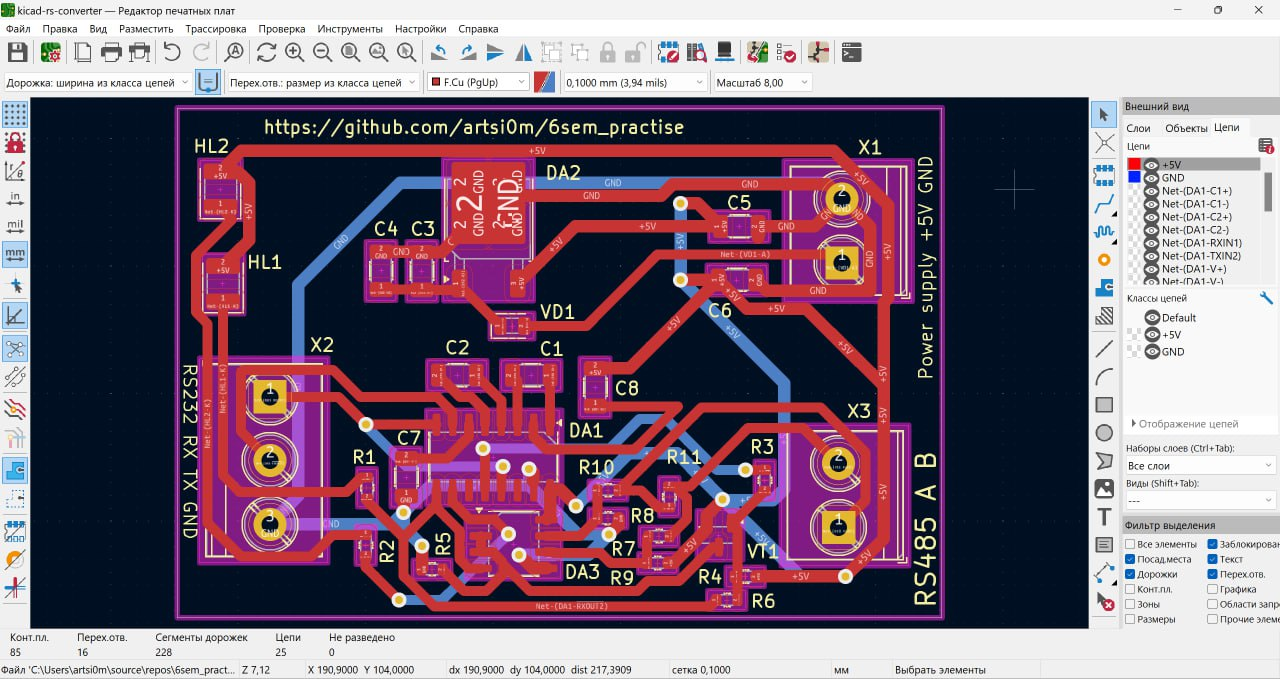
\includegraphics[scale=0.4]{kicad-pcb-doc-with-rs-converter.jpg}
  \caption{Снимок экрана с ПП открытой в kicad-pcbdoc}
\end{figure}


Эта программа, ныне одно из самых передовых решений,
среди всех свободных САПР ПП.

Примечательно также, что его разработку спонсировал
Европейский Институт Ядерных Исследований ~\cite{kicad-sponsors}.

Другая причина выбора данной САПР при разработке,
используемый в ней, текстовой формат файлов,
при котором данные в документах САПР представлены
не иначе как Эс-Выражения (англ. \textit{S-Expressions})
~\cite{kicad-sexpr}.

В отличие от бинарных файлов,
используемых в \textit{Altium Designer},
файлы созданные при разработке печатной платы,
в \textit{KiCAD} за счёт их использования текста
возможно разместить в репозитории git.

Git это распределённая система контроля версий 
исходного кода \cite{git-dvcs}.

Из-за формата,
файлы \textit{KiCAD} могут быть обработаны,
как исходный код.
Это даёт возможность удобной кооперации, при совместной работе.

\begin{figure}[H]
  \centering
  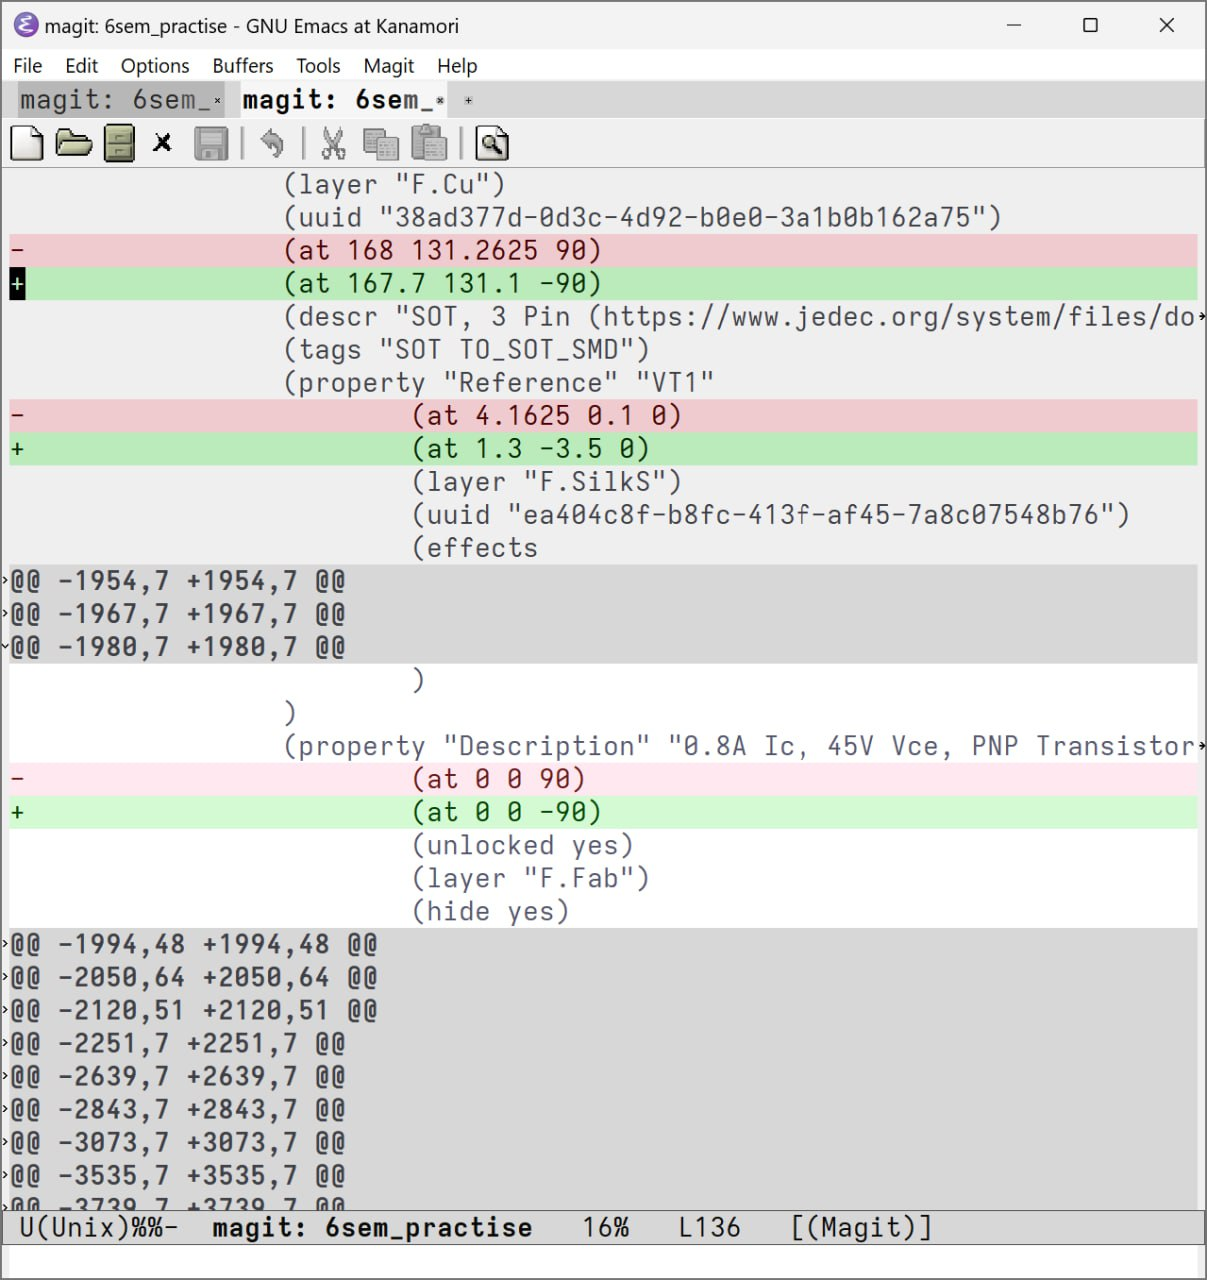
\includegraphics[scale=0.5]{magit-6-sem-practise.jpg}
  \caption{Снимок экрана с окном magit,
    установленный в расширяемый редактор текста GNU/Emacs
    клиент системы контроля версий git.
    Видно, как magit может распознать изменения файла трассировки печатной платы,
    как добавление и удаление строк.}
\end{figure}


Например в едимном репозитории печатной платы,
один конструктор в соотвествующем файле
создаёт принципиальную схему устройства,
а другой в свою очередь, синхронизировав файл
через \textit{git} , используя готовую схему
трассирует печатную плату.

Более того, используя, так называемый монорепозиторий, как подход работы с \textit{git},
в одном репозитории можно содержать как печатную плату,
так и исходный код прошивки микроконтроллера,
используемый в ней.

В данной САПР было осуществлено создание
принципиальной cхемы устройства,
а также трассировка печатной платы, на основе связей между элементами,
импортированных из схемотехнической
части программы \textit{kicad-eeschema} ~\cite{kicad-doc-eeschema}.

% SimulIDE, KTechLab Proteus

Во момент работы над принципиальной схемой, была
допущена ошибка, из-за которой транзистор,
был подключен не теми выводами,
которые были обозначены на взятой изначально принципиальный схеме.

О своей оплошности я был осведомлён уже в тот момент,
когда выслал файлы по почте в отдел производство.
Я был проинформирован о недочёте в схеме начальником производственного отдела.
Это дало мне ценный урок:
при любых сомнениях в схемотехнической части разрабатываемого устройства,
следует провести тестирование в САПР симуляторе.

Среди изученных мною ранее
таковой является \textit{Proteus} ~\cite{Proteus-Simulation}. Её аналог в мире свободного ПО - \textit{SimulIDE} ~\cite{SimulIDE}.
%

%\begin{figure}[H]
%  \centering
%  \includegraphics[scale=0.35]{SimulIDE.png}
%  \caption{Снимок экрана с окном САПР-симулятора SimulIDE}
%\end{figure}

Для разработки данной печатной платы было достаточно
использование САПР ПП \textit{KiCAD},
однако стоит отметить, что использование специальных САПР симуляторов,
например \textit{Proteus} или \textit{KiCAD} существенно бы ускорило,
процесс изготовления и введения устройства в эксплуатацию
за счёт экономии времени на этапе исправления ошибок в принципиальной схеме.

\newpage

% Local Variables:
% compile-command: "sh build.sh"
% End:
